%%%%%%%%%%%%%%%%%%%%%%%%%%%%%%%%%%%%%%%%%%%
%%%%%%%%%%%%%%%%%%%%%%%%%%%%%%%%%%%%%%%%%%%
%%%%%%%%%%%%%%% CHAPTER 02 %%%%%%%%%%%%%%%%


\section{Transformada de Laplace}

\frame{
\frametitle{Motivação}
\begin{block}{}
O foco principal do uso da \textbf{transformada de Laplace} neste curso é na análise de sistemas dinâmicos, sendo um método alternativo e eficaz para a resolução de EDOs.
\end{block}
}

\frame{
\frametitle{Por que usar a transformada de Laplace?}
\begin{block}{Vantagens}
\begin{itemize}
    \item A transformada de Laplace permite a conversão de equações diferenciais em \textbf{equações algébricas}, facilitando a sua manipulação.
    \item A solução completa é obtida em apenas um passo, diferentemente das EDOs.
    \item Não existem problemas com as condições iniciais em funções descontínuas.
\end{itemize}
\end{block}
}

\frame{
\frametitle{Definição}
\begin{block}{}
Considere uma função $f(t)$ definida nos reais não negativos. A sua transformada de Laplace é:
$$\boxed{\mathscr{L}\{f(t)\}=F(s) \triangleq \int_{0}^{\infty} f(t) \ e^{-st} \text{d}t}$$
\begin{itemize}
    \item Quando a integral for \textbf{convergente}, a transformada existe e é uma função de $s = \sigma + j \omega$, uma variável complexa.
    \item Letras minúsculas: funções do tempo.
    \item Letras maiúsculas: transformadas.
\end{itemize}
\end{block}
}

\frame{
\frametitle{Exemplo \#01 - Função degrau unitário}
\begin{block}{}
A função degrau unitário $r(t)$ é definida como sendo:
\begin{equation*}
r(t) \triangleq \begin{cases}
0 &\text{para $t < 0$}\\
1 &\text{para $t > 0$}\\
\text{não definida} &\text{para $t = 0$}
\end{cases}
\end{equation*}
\end{block}
\centerline{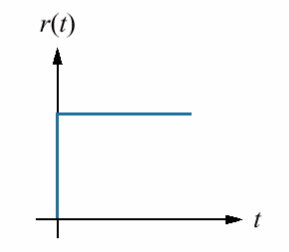
\includegraphics[width=0.4\linewidth]{Figuras/Ch02/fig1.PNG}}
}

\frame{
\frametitle{Exemplo \#01 - Função degrau unitário}
\begin{block}{Resolução}
$$\mathscr{L}\{r(t)\} = R(s) = \int_{0}^{\infty} 1 \ e^{-st} \text{d}t = - \dfrac{e^{-st}}{s} \bigg\rvert_{0}^{\infty} = - \dfrac{e^{-(\sigma + j \omega)\infty}}{s} + \dfrac{e^{-(\sigma + j \omega)0}}{s}$$
\begin{itemize}
    \item Para $\sigma > 0$, temos  $\mathscr{L}\{r(t)\}=R(s) = \dfrac{1}{s}$
    \item Para $\sigma < 0$, temos que a integral é divergente.
\end{itemize}
\end{block}
}

\frame{
\frametitle{Exemplo \#02 - Função rampa unitária}
\begin{block}{}
A função rampa unitária $r(t)$ é definida como sendo:
\begin{equation*}
r(t) \triangleq \begin{cases}
0 &\text{para $t \leq 0$}\\
t &\text{para $t > 0$}
\end{cases}
\end{equation*}
\end{block}
\centerline{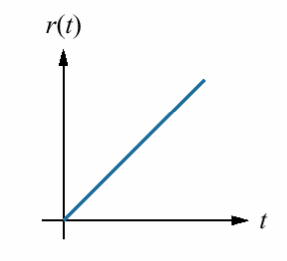
\includegraphics[width=0.4\linewidth]{Figuras/Ch02/fig2.PNG}}
}

\frame{
\frametitle{Exemplo \#02 - Função rampa unitária}
\begin{block}{Resolução}
$$\mathscr{L}\{r(t)\}=R(s) = \int_{0}^{\infty} t \ e^{-st} \text{d}t = -t \dfrac{e^{-st}}{s} \bigg\rvert_{0}^{\infty} + \dfrac{1}{s} \int_{0}^{\infty} e^{-st} \text{d}t$$ \\
$$\boxed{\int_{0}^{\infty} u \ \text{d}v = uv\bigg\rvert_{0}^{\infty} - \int_{0}^{\infty} v \ \text{d}u}$$
\begin{itemize}
    \item Para $\sigma > 0$, temos  $\mathscr{L}\{r(t)\} = R(s) = 0 - 0 + \dfrac{1}{s} \mathscr{L}\{1\} = \dfrac{1}{s^2}$
    \item Para $\sigma < 0$, temos que a integral é divergente.
\end{itemize}
\end{block}
}

\frame{
\frametitle{Exemplo \#03 - Função parábola unitária}
\begin{block}{}
A função parábola unitária $r(t)$ é definida como sendo:
\begin{equation*}
r(t) \triangleq \begin{cases}
0 &\text{para $t \leq 0$}\\
\frac{1}{2}t^2 &\text{para $t > 0$}
\end{cases}
\end{equation*}
\end{block}
\centerline{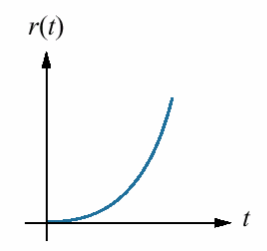
\includegraphics[width=0.4\linewidth]{Figuras/Ch02/fig3.PNG}}
}

\frame{
\frametitle{Exemplo \#03 - Função parábola unitária}
\begin{block}{Resolução}
$$\mathscr{L}\{r(t)\}=R(s) = \int_{0}^{\infty} \frac{1}{2}t^2 \ e^{-st} \text{d}t = -\frac{1}{2}t^2 \dfrac{e^{-st}}{s} \bigg\rvert_{0}^{\infty} + \dfrac{1}{s} \int_{0}^{\infty} t \ e^{-st} \text{d}t$$ \\
$$\boxed{\int_{0}^{\infty} u \ \text{d}v = uv\bigg\rvert_{0}^{\infty} - \int_{0}^{\infty} v \ \text{d}u}$$
\begin{itemize}
    \item Para $\sigma > 0$, temos  $\mathscr{L}\{r(t)\} = R(s) = 0 - 0 + \dfrac{1}{s} \mathscr{L}\{t\} = \dfrac{1}{s^3}$
    \item Para $\sigma < 0$, temos que a integral é divergente.
\end{itemize}
\end{block}
}

\frame{
\frametitle{Exemplo \#04 - Função $r(t) = t^n$}
\begin{block}{Resolução}
Lembrando que:
\begin{itemize}
    \item $r(t) = 1 \implies R(s) = \frac{1}{s}$
    \item $r(t) = t \implies R(s) = \frac{1}{s^2}$
    \item $r(t) = \frac{1}{2}t^2 \implies R(s) = \frac{1}{s^3}$ \\
\end{itemize}
\vspace{0.5cm}
De maneira intuitiva, temos que para $r(t) = t^n$ usamos a ideia introduzida nos exemplos anteriores e escrevemos a sua transformada em termos da transformada de $t^{n-1}$.
Portanto, 
\begin{itemize}
    \item Para $\sigma > 0$, temos  $\mathscr{L}\{r(t)\} = R(s) = \dfrac{n!}{s^{n+1}}$
    \item Para $\sigma < 0$, temos que a integral é divergente.
\end{itemize}
\end{block}
}

\frame{
\frametitle{Exemplo \#05 - Função $r(t) = e^{-at}$}
\begin{block}{Resolução}
$$\mathscr{L}\{r(t)\}=R(s) = \int_{0}^{\infty} e^{-at} \ e^{-st} \text{d}t =  \int_{0}^{\infty} e^{-(s+a)t} \text{d}t = -\frac{1}{s+a} \ e^{-(s+a)t}\bigg\rvert_{0}^{\infty}$$ \\
\begin{itemize}
    \item Para $\sigma + a > 0$, temos  $\mathscr{L}\{r(t)\} = R(s) = -\dfrac{1}{s+a}\Big(0 - 1 \Big) = \dfrac{1}{s+a}$
    \item Para $\sigma + a < 0$, temos que a integral é divergente.
\end{itemize}
\end{block}
}

\frame{
\frametitle{Exemplo \#06 - Função $r(t) = \text{sen}(\omega t)$}
\begin{block}{Resolução}
$$ \mathscr{L}\{r(t)\}=R(s) = \int_{0}^{\infty} \text{sen}(\omega t) \ e^{-st} \text{d}t = -\frac{\text{sen}(\omega t) \ e^{-st}}{s} \bigg\rvert_{0}^{\infty} +$$
$$+ \dfrac{\omega}{s} \int_{0}^{\infty} \text{cos}(\omega t) \ e^{-st} \text{d}t = 0 - 0 + \frac{\omega}{s} \int_{0}^{\infty} \text{cos}(\omega t) \ e^{-st} \text{d}t $$ 
$$\mathscr{L}\{r(t)\}=R(s)  = \frac{\omega}{s}\Bigg[-\frac{\text{cos}(\omega t) \ e^{-st}}{s} \bigg\rvert_{0}^{\infty} - \dfrac{\omega}{s} \int_{0}^{\infty} \text{sen}(\omega t) \ e^{-st} \text{d}t\Big]$$ 
$$\mathscr{L}\{r(t)\}=R(s) = \frac{\omega}{s}\Bigg[0 - \Big(-\frac{1}{s}\Big) - \dfrac{\omega}{s} \int_{0}^{\infty} \text{sen}(\omega t) \ e^{-st} \text{d}t\Big] = \frac{\omega}{s^2} - \frac{\omega^2}{s^2} \ \mathscr{L}\{r(t)\}$$ 
\begin{itemize}
    \item Para $\sigma > 0$, temos  $\mathscr{L}\{r(t)\} = R(s) = \dfrac{\omega}{s^2 + \omega^2}$
    \item Para $\sigma < 0$, temos que a integral é divergente.
\end{itemize}
\end{block}
}

\frame{
\frametitle{Exemplo \#07 - Função definida por partes}
\begin{block}{}
Considere uma função $r(t)$ definida por partes:
\begin{equation*}
r(t) =\begin{cases}
0 &\text{para $0 \leq t \leq 4$}\\
5 &\text{para $t > 4$}\\
\end{cases}
\end{equation*}
\end{block}
}

\frame{
\frametitle{Exemplo \#07 - Função definida por partes}
\begin{block}{Resolução}
$$\mathscr{L}\{r(t)\}=R(s) = \int_{0}^{\infty} r(t) \ e^{-st} \text{d}t = \int_{0}^{4} r(t) \ e^{-st} \text{d}t + \int_{4}^{\infty} r(t) \ e^{-st} \text{d}t$$ \\
$$\boxed{\int_{a}^{b} r(t) \ \text{d}t = \int_{a}^{x} r(t) \ \text{d}t + \int_{x}^{b} r(t) \ \text{d}t}$$
$$\mathscr{L}\{r(t)\}=R(s) = \int_{0}^{4} 0 \ e^{-st} \text{d}t + \int_{4}^{\infty} 5 \ e^{-st} \text{d}t$$ 
\begin{itemize}
    \item Para $\sigma > 0$, temos  $\mathscr{L}\{r(t)\} = R(s) = \dfrac{5 \ e^{-4s}}{s}$
    \item Para $\sigma < 0$, temos que a integral é divergente.
\end{itemize}
\end{block}
}

\frame{
\frametitle{Condições de existência da transformada de Laplace}
\begin{block}{Introdução}
A integral que define a transformada de Laplace nem sempre converge e, nesse caso, dizemos que a função não possui transformada de Laplace. As funções $f(t) = \text{e}^{t^2}$ e $f(t) = 1/t$ são alguns exemplos de funções que não possuem transformada de Laplace. 
\end{block}
}

\frame{
\frametitle{Condições de existência da transformada de Laplace}
\begin{block}{Condições}
As \textbf{condições suficientes} para existência da transformada de Laplace são:

\begin{enumerate}
    \item a função é contínua por partes;
    \item a função é de ordem exponencial;
    \item a função é definida apenas para $t>0$.
\end{enumerate}

\textbf{Estas condições não são, no entanto, necessárias}.

\begin{itemize}
    \item Por exemplo, a função $f(t) = \text{ln}(t)$ não é contínua na origem, sequer é limitada quando $t \to 0^+$, mas admite uma transformada de Laplace.
\end{itemize}
\end{block}
}

\frame{
\frametitle{Condições de existência da transformada de Laplace}
\begin{block}{A função é contínua por partes}
Uma função $f(t)$ é \textbf{contínua por partes} no intervalo $[0, \infty]$ se esta, em qualquer
intervalo $0 \leq a \leq t \leq b$, tiver um número finito de descontinuidade e toda
descontinuidade for de primeira espécie, isto é, se os limites laterais de $f(t)$ existirem (são finitos) e se forem distintos.
\end{block}
\vspace{0.3cm}
\centerline{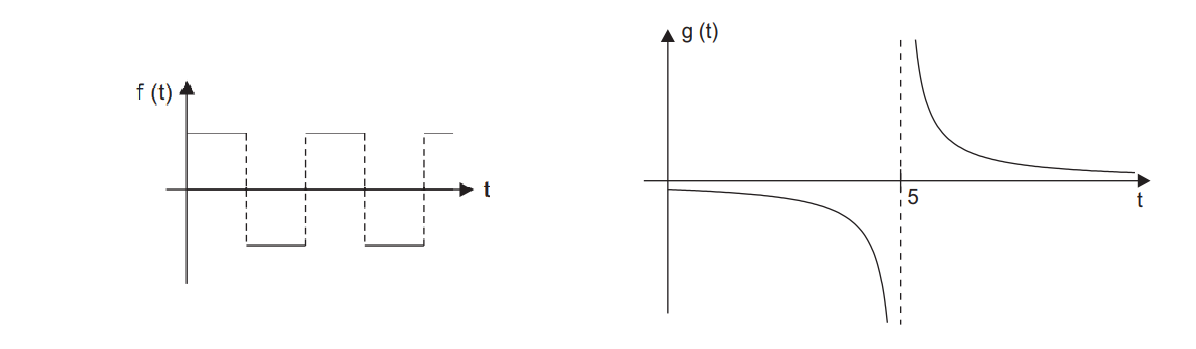
\includegraphics[width=1.1\linewidth]{Figuras/Ch02/fig4.PNG}}
}

\frame{
\frametitle{Condições de existência da transformada de Laplace}
\begin{block}{A função é de ordem exponencial}
Dizemos que uma função $f(t)$ é de \textbf{ordem exponencial} $c$ se existem constantes $c$, $M > 0$ e $T > 0$ tal que $|f(t)| \leq M e^{ct}$ para todo $t > T$.
\begin{itemize}
    \item $f(t) = t^2$ é de ordem exponencial pois $|t^2| \leq e^t$, $t>0$
    \item $g(t) = 5 \ \text{cos}(t)$ é de ordem exponencial pois $|5 \ \text{cos}(t)| \leq e^t$, $t>1$
    \item $h(t) = e^{-t}$ é de ordem exponencial pois $|e^{-t}| \leq e^t$, $t>0$
\end{itemize}
\end{block}
\vspace{0.3cm}
\centerline{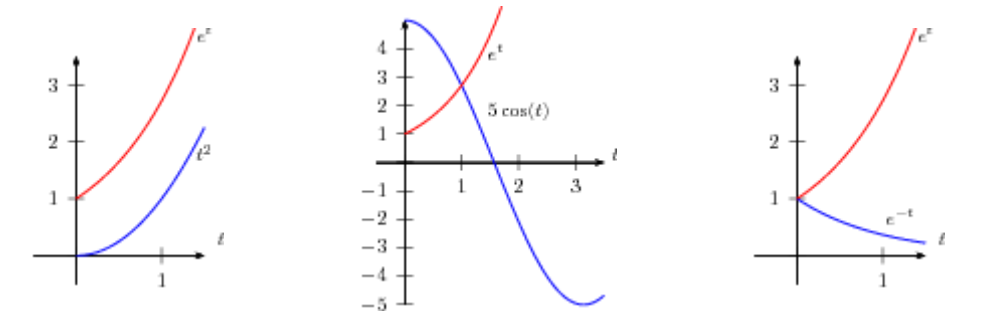
\includegraphics[width=1\linewidth]{Figuras/Ch02/fig5.PNG}}
}

\frame{
\frametitle{Condições de existência da transformada de Laplace}
\begin{block}{A função é definida apenas para $t>0$}
A condição de $f(t) = 0$ para $t < 0$ é explicita por si só, mas é comum a \textbf{falta de rigor neste requisito}. 
\begin{itemize}
    \item Exemplificando, a função $f(t) = \text{cos}(\omega t)$ não é transformável porque ela não é nula para $t < 0$.
    \item O instante admitido como $t = 0$ é uma
    questão de escolha; portanto, a exigência de $f(t) = 0$ para $t < 0$ \textbf{não representa uma restrição}.
\end{itemize}
\end{block}
\centerline{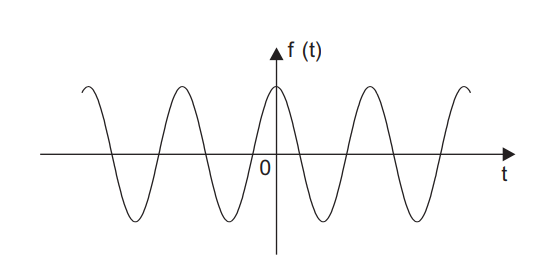
\includegraphics[width=0.6\linewidth]{Figuras/Ch02/fig6.PNG}}
}

\frame{
\frametitle{Condições de existência da transformada de Laplace}
\begin{block}{Teorema}
\textbf{Teorema}: Se $f(t)$ é integrável em cada intervalo $[a,b] \in [0,\infty)$ e de ordem exponencial $c$, então a transformada de Laplace de $f(t)$ existe para $s>c$. \\
\vspace{0.2cm}
\textbf{Demonstração}: Como a função $f(t)$ é de ordem exponencial $c$, então existem constantes $c$, $M > 0$ e $T > 0$ tal que $|f(t)| \leq M e^{ct}$ para todo $t > T$. Assim, se $\hat{T}$ é maior ou igual a $T$, a transformada de Laplace pode ser escrita como a seguinte soma:
$$\mathscr{L}\{f(t)\} = \int_{0}^{\infty} f(t) \ e^{-st} \text{d}t = \int_{0}^{\hat{T}} f(t) \ e^{-st} \text{d}t + \int_{\hat{T}}^{\infty} f(t) \ e^{-st} \text{d}t $$
A primeira parcela do lado direito é a integral do produto de duas funções integráveis no intervalo $[0,\hat{T}]$, logo está bem definida (integral própria).
\end{block}
}

\frame{
\frametitle{Condições de existência da transformada de Laplace}
\begin{block}{Teorema}
Agora, como $\hat{T} \geq T$, podemos estimar
$$\Big|\int_{\hat{T}}^{\infty} f(t) \ e^{-st} \text{d}t \Big| \leq \int_{\hat{T}}^{\infty} |f(t)| \ e^{-st} \text{d}t \leq \int_{\hat{T}}^{\infty} M e^{ct} \ e^{-st} \text{d}t =$$
$$= M \int_{\hat{T}}^{\infty} e^{-(s-c)t} \text{d}t = \frac{M}{c-s} \ e^{-(s-c)t}\bigg\rvert_{\hat{T}}^{\infty} = \frac{M}{c-s} \ e^{-(s-c)\hat{T}} \quad s > c$$
A integral $\mathscr{L}\{f(t)\} = \int_{0}^{\infty} f(t) \ e^{-st} \text{d}t$ converge para todo $s>c$, ou seja, a transformada de Laplace existe neste domínio. \qed
\end{block}
}

\frame{
\frametitle{Propriedades}
\begin{block}{Superposição}
Considere uma função $f(t)$ cuja transformada de Laplace é $F(s)$, e considere ainda uma função $g(t)$ cuja transformada de Laplace é $G(s)$. Deste modo:

$$\mathscr{L}\{\alpha f(t) + \beta g(t)\} = \alpha F(s) + \beta G(s)$$ \\
\vspace{0.2cm}
\textbf{Demonstração}: 
$$\mathscr{L}\{\alpha f(t) + \beta g(t)\} = \int_{0}^{\infty} [\alpha f(t) + \beta g(t)] \ e^{-st} \text{d}t =$$
$$= \alpha \int_{0}^{\infty} f(t) \ e^{-st} \text{d}t + \beta \int_{0}^{\infty} g(t) \ e^{-st} \text{d}t = \alpha F(s) + \beta G(s)$$ \qed
\end{block}
}

\frame{
\frametitle{Propriedades}
\begin{block}{Superposição - Exemplo}
$$\mathscr{L}\{4t^2 - 3 \ \text{cos}(t) + 5 \ e^{-t}\} = 4 \mathscr{L}\{t^2\} -3 \mathscr{L}\{\text{cos}(t)\} + 5 \mathscr{L}\{e^{-t}\} =$$
$$= 4 \ \frac{2!}{s^3} - 3 \ \frac{s}{s^2 + 1} + 5 \ \frac{1}{s+1} = \frac{8}{s^3} - \frac{3s}{s^2 + 1} + \frac{5}{s+1}$$
\end{block}
}

\frame{
\frametitle{Propriedades}
\begin{block}{Escalamento temporal (contração)}
Se $\mathscr{L}\{f(t)\} = F(s)$, então $\mathscr{L}\{f(at)\} = \frac{1}{a}F\Big(\frac{s}{a}\Big)$ \\
\vspace{0.2cm}
\textbf{Demonstração}: Seja $at = u$, então:
$$\mathscr{L}\{f(at)\} = \int_{0}^{\infty} f(at) \ e^{-st} \text{d}t =$$
$$= \int_{0}^{\infty} f(u) \ e^{-s \frac{u}{a}} \frac{\text{d}u}{a} = \frac{1}{a} \int_{0}^{\infty} f(u) \ e^{-\frac{s}{a}u} \text{d}u = \frac{1}{a}F\Big(\frac{s}{a}\Big)$$ \qed \\
\vspace{0.2cm}
\textbf{Corolário}: contração no tempo equivale a expansão na frequência, e vice-versa.
\end{block}
}

\frame{
\frametitle{Propriedades}
\begin{block}{Escalamento temporal (contração) - Exemplo}
Como $\mathscr{L}\{\text{sen}(t)\} = \dfrac{1}{s^2 + 1}$, temos que
$$\mathscr{L}\{\text{sen}(3t)\} = \frac{1}{3}F\Big(\frac{s}{3}\Big) = \frac{1}{3} \frac{1}{(\frac{s}{3})^2 + 1} = \frac{1}{3} \frac{9}{s^2 + 9} = \frac{3}{s^2 + 9}$$
\end{block}
}

\frame{
\frametitle{Propriedades}
\begin{block}{Deslocamento no tempo}
Se $\mathscr{L}\{f(t)\} = F(s)$, então $\mathscr{L}\{f(t-a)\} = e^{-sa}F(s)$ \\
\vspace{0.2cm}
\textbf{Demonstração}: Seja $t - a = \gamma$, então:
$$\mathscr{L}\{f(t-a)\} = \int_{0}^{\infty} f(t-a) \ e^{-st} \text{d}t =$$
$$= \int_{0}^{\infty} f(\gamma) \ e^{-s(\gamma + a)} \text{d}\gamma = e^{-sa} \int_{0}^{\infty} f(\gamma) \ e^{-s \gamma} \text{d}\gamma = e^{-sa} F(s)$$ \qed \\
\end{block}
}

\frame{
\frametitle{Propriedades}
\begin{block}{Deslocamento no tempo - Exemplo}
Como $\mathscr{L}\{1\} = \dfrac{1}{s}$, temos que
$$\mathscr{L}\{1(t-2)\} = e^{-2s} F(s) =  \dfrac{e^{-2s}}{s}$$
\end{block}
}

\frame{
\frametitle{Propriedades}
\begin{block}{Multiplicação por uma exponencial}
Se $\mathscr{L}\{f(t)\} = F(s)$, então $\mathscr{L}\{e^{-at}f(t)\} = F(s+a)$ \\
\vspace{0.2cm}
\textbf{Demonstração}:
$$\mathscr{L}\{e^{-at}f(t)\} = \int_{0}^{\infty} e^{-at}f(t) \ e^{-st} \text{d}t =$$
$$= \int_{0}^{\infty} f(t) \ e^{-(s + a)t} \text{d}t = F(s + a)$$ \qed \\
\vspace{0.2cm}
\textbf{Corolário}: estas duas últimas propriedades são duais uma da outra pois enquanto uma diz que a transformada do sinal transladado no tempo fica multiplicada por uma exponencial na frequência, a outra diz que a transformada de um sinal multiplicado por uma exponencial no tempo é um sinal transladado na frequência. 
\end{block}
}

\frame{
\frametitle{Propriedades}
\begin{block}{Multiplicação por uma exponencial - Exemplo}
Como $\mathscr{L}\{\text{sen}(\omega t)\} = \dfrac{\omega}{s^2 + \omega^2}$, temos que
$$\mathscr{L}\{e^{-4t} \text{sen}(\omega t)\} = F(s + 4) = \dfrac{\omega}{(s+4)^2 + \omega^2}$$
\end{block}
}

\frame{
\frametitle{Propriedades}
\begin{block}{Multiplicação pelo tempo}
Se $\mathscr{L}\{f(t)\} = F(s)$, então $\mathscr{L}\{tf(t)\} = -\dfrac{\text{d}}{\text{d}s}F(s)$ \\
\vspace{0.2cm}
\textbf{Demonstração}:
$$\dfrac{\text{d}}{\text{d}s}F(s) = \dfrac{\text{d}}{\text{d}s}\int_{0}^{\infty} f(t) \ e^{-st} \text{d}t = \int_{0}^{\infty} \dfrac{\partial}{\partial s} \left[f(t) \ e^{-st}\right] \text{d}t =$$
$$= \int_{0}^{\infty} -tf(t) \ e^{-st} \text{d}t = - \mathscr{L}\{tf(t)\}$$ \qed \\
\end{block}
}

\frame{
\frametitle{Propriedades}
\begin{block}{Multiplicação pelo tempo - Exemplo}
Como $\mathscr{L}\{1\} = \dfrac{1}{s}$, temos que
$$\mathscr{L}\{t\} = -\dfrac{\text{d}}{\text{d}s}\left(\dfrac{1}{s}\right)=\dfrac{1}{s^2}$$
\end{block}
}

\frame{
\frametitle{Teoremas}
\begin{block}{Teorema da derivação real}
Se $\mathscr{L}\{f(t)\} = F(s)$, então $\mathscr{L}\{\dot{f}(t)\} = sF(s) - f(0)$ \\
\vspace{0.2cm}
\textbf{Demonstração}:
$$\mathscr{L}\{\dot{f}(t)\} = \int_{0}^{\infty} \dot{f}(t) \ e^{-st} \text{d}t = e^{-st} f(t)\bigg\rvert_{0}^{\infty} + s\int_{0}^{\infty} f(t) \ e^{-st} \text{d}t$$
$$\boxed{\int_{0}^{\infty} u \ \text{d}v = uv\bigg\rvert_{0}^{\infty} - \int_{0}^{\infty} v \ \text{d}u}$$
$$\mathscr{L}\{\dot{f}(t)\} = [0 - f(0)]+ s\int_{0}^{\infty} f(t) \ e^{-st} \text{d}t = sF(s) - f(0)$$ \qed
\end{block}
}

\frame{
\frametitle{Teoremas}
\begin{block}{Teorema da derivação real - ordem superior}
Se $\mathscr{L}\{\dot{f}(t)\} = sF(s) - f(0)$, então $\mathscr{L}\{\ddot{f}(t)\} = s^2F(s) - sf(0) - \dot{f}(0)$ \\
\vspace{0.2cm}
\textbf{Demonstração}:
$$\mathscr{L}\{\ddot{f}(t)\} = s \mathscr{L}\{\dot{f}(t)\} - \dot{f}(0) = s[sF(s) - f(0)] - \dot{f}(0) = s^2F(s) - sf(0) - \dot{f}(0)$$ \qed \\
\vspace{0.2cm}
\textbf{Corolário}: (Generalização) Seja $\mathscr{L}\{f(t)\} = F(s)$, então
$$\mathscr{L}\{f^{(n)}(t)\} = s^n F(s) - s^{n-1}f(0) - s^{n-2}\dot{f}(0) - ... - sf^{(n-2)}(0) - f^{(n-1)}(0)$$
\end{block}
}

\frame{
\frametitle{Teoremas}
\begin{block}{Teorema da integração real}
Se $\mathscr{L}\{f(t)\} = F(s)$, então $\mathscr{L}\{\int_{0}^{t} f(u) \text{d}u \} = \dfrac{F(s)}{s}$ \\
\vspace{0.2cm}
\textbf{Demonstração}:
$$g(t) = \int_{0}^{t} f(u) \text{d}u \implies \dot{g}(t) = f(t)$$
$$\mathscr{L}\{\dot{g}(t)\} = \mathscr{L}\{f(t)\} \implies s \mathscr{L}\{g(t)\} - g(0) = F(s) \implies s \mathscr{L}\{g(t)\} = F(s)$$
$$\mathscr{L}\{g(t)\} = \dfrac{F(s)}{s} \implies \mathscr{L}\left\{\int_{0}^{t} f(u) \text{d}u \right\} = \dfrac{F(s)}{s}$$ \qed
\end{block}
}

\frame{
\frametitle{Teoremas}
\begin{block}{Teorema do valor final}
Se os limites indicados existem, então $\lim_{t\to\infty} f(t) = \lim_{s\to 0} sF(s)$ \\
\vspace{0.2cm}
\textbf{Demonstração}:
$$\mathscr{L}\{\dot{f}(t)\} = \int_{0}^{\infty} \dot{f}(t) \ e^{-st} \text{d}t = sF(s) - f(0)$$ 
Tomando os limites de ambos os lados quando $s \to 0$, temos
$$\lim_{s\to 0} \int_{0}^{\infty} \dot{f}(t) \ e^{-st} \text{d}t = \lim_{s\to 0} [sF(s) - f(0)]$$
$$\int_{0}^{\infty} \dot{f}(t) \text{d}t = \lim_{s\to 0} [sF(s)] - f(0)$$
$$[f(\infty) - f(0)] = \lim_{s\to 0} [sF(s)] - f(0) \implies \lim_{t\to\infty} f(t) = \lim_{s\to 0} sF(s)$$ \qed
\end{block}
}

\frame{
\frametitle{Teoremas}
\begin{block}{Teorema do valor inicial}
Se os limites indicados existem, então $\lim_{t\to 0} f(t) = \lim_{s\to \infty} sF(s)$ \\
\vspace{0.2cm}
\textbf{Demonstração}:
$$\mathscr{L}\{\dot{f}(t)\} = \int_{0}^{\infty} \dot{f}(t) \ e^{-st} \text{d}t = sF(s) - f(0)$$ 
Tomando os limites de ambos os lados quando $s \to \infty$, temos
$$\lim_{s\to \infty} \int_{0}^{\infty} \dot{f}(t) \ e^{-st} \text{d}t = \lim_{s\to \infty} [sF(s) - f(0)]$$
$$0 = \lim_{s\to \infty} [sF(s)] - f(0)$$
$$f(0) = \lim_{s\to \infty} sF(s) \implies \lim_{t\to 0} f(t) = \lim_{s\to \infty} sF(s)$$ \qed
\end{block}
}

\begin{frame}[allowframebreaks]{Tabela de transformadas}
\begin{longtable}{cc}
	$ f(t)=\mathscr{L}^{-1}\{F(s)\} $ & $ F(s)=\mathscr{L}\{f(t)\} $\\\addlinespace\toprule\addlinespace
	$\delta (t)$ & $ 1 $
	\\\addlinespace\midrule\addlinespace[0.2cm]
	$\dot{\delta}(t)$ & $s$
	\\\addlinespace\midrule\addlinespace[0.2cm]
	$ 1 $ & $ 1/s $ \\\addlinespace\midrule\addlinespace[0.2cm]
	$ e^{at} $ & $ 1/(s-a) $\\\addlinespace\midrule\addlinespace[0.2cm]
	$ t^{n} $, $ n=1,2,3,\ldots $ & $ \dfrac{n!}{s^{n+1}} $\\\addlinespace\midrule\addlinespace[0.2cm]
	$ t^{p} $, $ p>-1 $ & $ \dfrac{\Gamma \left(p + 1\right)}{s^{p + 1}} $\\\addlinespace\midrule\addlinespace[0.2cm]
	$ \sqrt{t} $ & $ \dfrac{\sqrt{\pi}}{2s^{\sfrac{3}{2}}} $\\\addlinespace\midrule\addlinespace[0.2cm]
	$ t^{n-\sfrac{1}{2}} $, $ n=1,2,3,\ldots $ & $ \dfrac{1\cdot3\cdot5\cdots(2n-1)\sqrt{\pi}}{2^{n}s^{n+\sfrac{1}{2}}} $
	\\\addlinespace\midrule\addlinespace[0.2cm]
	$ \sin{at} $ & $ \dfrac{a}{s^{2}+a^{2}} $\\\addlinespace\midrule\addlinespace[0.2cm]
	$ \cos{at} $ & $ \dfrac{s}{s^{2}+a^{2}} $\\\addlinespace\midrule\addlinespace[0.2cm]
	$ t\sin{at} $ & $ \dfrac{2as}{\left(s^{2}+a^{2}\right)^{2}} $\\\addlinespace\midrule\addlinespace[0.2cm]
	$ t\cos{at} $ & $ \dfrac{s^{2}-a^{2}}{\left(s^{2}+a^{2}\right)^{2}} $\\\addlinespace\midrule\addlinespace[0.2cm]
	$ \sin{at}-at\cos{at} $ & $ \dfrac{2a^{3}}{\left(s^{2}+a^{2}\right)^{2}} $\\\addlinespace\midrule\addlinespace[0.2cm]
	$ \sin{at}+at\cos{at} $ & $ \dfrac{2as^{2}}{\left(s^{2}+a^{2}\right)^{2}} $
	\\\addlinespace\midrule\addlinespace[0.2cm]
	$ \cos{at}-at\sin{at} $ & $ \dfrac{s\left(s^{2}-a^{2}\right)}{\left(s^{2}+a^{2}\right)^{2}} $\\\addlinespace\midrule\addlinespace[0.2cm]
	$ \cos{at}+at\sin{at} $ & $ \dfrac{s\left(s^{2}+3a^{2}\right)}{\left(s^{2}+a^{2}\right)^{2}} $\\\addlinespace\midrule\addlinespace[0.2cm]
	$ \sin{at+b} $ & $ \dfrac{s\sin{b}+a\cos{b}}{s^{2}+a^{2}} $\\\addlinespace\midrule\addlinespace[0.2cm]
	$ \cos{at+b} $ & $ \dfrac{s\cos{b}-a\sin{b}}{s^{2}+a^{2}} $\\\addlinespace
	$ \sinh{at} $ & $ \dfrac{a}{s^{2}-a^{2}} $\\\addlinespace\midrule\addlinespace[0.2cm]
	$ \cosh{at} $ & $ \dfrac{s}{s^{2}-a^{2}} $\\\addlinespace\midrule\addlinespace[0.2cm]
	$ e^{at}\sin{bt} $ & $ \dfrac{b}{\left(s-a\right)^{2}+b^{2}} $\\\addlinespace\midrule\addlinespace[0.2cm]
	$ e^{at}\cos{bt} $ & $ \dfrac{s-a}{\left(s-a\right)^{2}+b^{2}} $\\\addlinespace\midrule\addlinespace[0.2cm]
	$ e^{at}\sinh{bt} $ & $ \dfrac{b}{\left(s-a\right)^{2}-b^{2}} $\\\addlinespace\midrule\addlinespace[0.2cm]
	$ e^{at}\cosh{bt} $ & $ \dfrac{s-a}{\left(s-a\right)^{2}-b^{2}} $\\\addlinespace\midrule\addlinespace[0.2cm]
	$ t^{n}e^{at} $,$ n=1,2,3,\ldots $ & $ \dfrac{n!}{\left(s-a\right)^{n+1}} $\\\addlinespace\midrule\addlinespace[0.2cm]
	$ f(ct) $ & $ \dfrac{1}{c}F\left( \dfrac{s}{c} \right)  $\\\addlinespace\midrule\addlinespace[0.2cm]
	$ u_{c}(t)=t(t-c) $ & $ \dfrac{c^{-cs}}{s} $\\\addlinespace\midrule\addlinespace[0.2cm]
	$ \delta(t-c) $ & $ e^{-cs} $\\\addlinespace\midrule\addlinespace[0.2cm]
	$ u_{c}(t)f(t-c) $ & $ e^{-cs}F(s) $\\\addlinespace\midrule\addlinespace[0.2cm]
	$ e_{c}(t)g(t) $ & $ e^{-cs}\mathscr{L}\{f(t+c)\} $\\\addlinespace\midrule\addlinespace[0.2cm]
	$ e^{ct}f(t) $ & $ F(s-c) $\\\addlinespace[0.2cm]\midrule\addlinespace[0.2cm]
	$ t^{n}f(t) $, $ n=1,2,3,\ldots $ & $ (-1)^{n}F^{(n)}(s)  $\\\addlinespace
	$ \dfrac{1}{t}f(t) $ & $ \displaystyle \int_{s}^{\infty}F(u)du $\\\addlinespace\midrule\addlinespace[0.2cm]
	$ \displaystyle \int_{0}^{t}f(v)dv $ & $ \dfrac{F(s)}{s}  $\\\addlinespace\midrule\addlinespace[0.2cm]
	$ \displaystyle\int_{0}^{t}f(t-\tau)g(\tau)d\tau $ & $F(s)G(s)  $\\\addlinespace\midrule\addlinespace[0.2cm]
	$ f^\prime(t) $ & $ sF(s)-f(0) $\\\addlinespace[0.2cm]\midrule\addlinespace[0.2cm]
	$ f^{\prime\prime}(t) $ & $ s^{2}F(s)-sf(0)-f^\prime(0) $\\\addlinespace\midrule\addlinespace[0.2cm]
	$ f^{(n)}(t) $ & $\begin{array} {c@{}l@{}} s^{n}F(s)- s^{n-1}f(0)-s^{n-2}f^\prime(0)&{}\cdots\\-sf^{(n-2)}(0)-f^{(n-1)}(0)& \end{array}$ \\\bottomrule
\end{longtable}
\end{frame}

\cprotect\frame{
\frametitle{\MATLAB}
\begin{block}{}
\begin{verbatim}
>>laplace(f)
\end{verbatim}
retorna a transformada de Laplace de $\bm{f}$. Por padrão, a variável independente é $ \bm{t} $ e variável de transformação é $ \bm{s} $. \\
\vspace{0.2cm}
\textbf{Exemplo}: calcule a transformada de Laplace de $e^{-at}$
\end{block}
\centerline{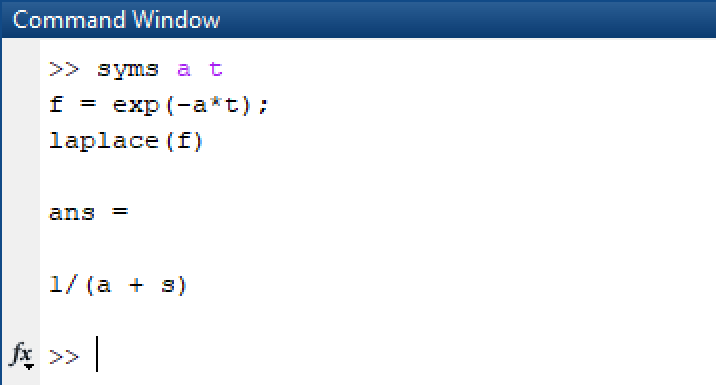
\includegraphics[width=0.7\linewidth]{Figuras/Ch02/fig10.PNG}}
}

\frame{
\frametitle{Exercícios}
\begin{block}{}
01. Calcule a transformada de Laplace da função $f(t) = \text{cos}(\omega t)$ usando a definição.

\vspace{1cm}

02. Calcule a transformada de Laplace da função $f(t)$ definida por partes:
\begin{equation*}
f(t) =\begin{cases}
0 &\text{para $0 \leq t \leq 3$}\\
1 &\text{para $3 < t \leq 5$}\\
0 &\text{para $t > 5$}\\
\end{cases}
\end{equation*}

\end{block}
}

\frame{
\frametitle{Exercícios}
\begin{block}{}
03. Considere a função pulso retangular de amplitude $A$ e duração $L$ mostrada na figura abaixo. Determine sua transformada de Laplace e, em seguida, mostre que quando $A = 1$ e $L \to \infty$, esta transformada é idêntica à transformada de Laplace do degrau unitário.
\end{block}
\vspace{0.2cm}
\centerline{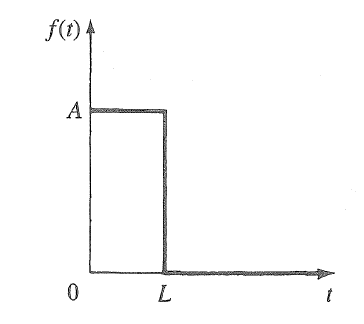
\includegraphics[width=0.5\linewidth]{Figuras/Ch02/fig11.PNG}}
}

\frame{
\frametitle{Exercícios}
\begin{block}{}
04. Demonstre a propriedade do escalamento temporal (expansão): \\
Se $\mathscr{L}\{f(t)\} = F(s)$ então $\mathscr{L}\{f(\frac{t}{a})\} = a F(as)$

\vspace{1cm}

05. Mostre por recursividade: $\mathscr{L}\{\dddot{f}(t)\} = s^3F(s) - s^2f(0) - s\dot{f}(0) - \ddot{f}(0)$

\vspace{1cm}

06. Utilizando o teorema do valor final e o teorema do valor inicial, encontre $f(0)$ e $f(\infty)$ para $f(t) = 5e^{-2t}$
\end{block}
}

\frame{
\frametitle{Referências e exercícios complementares}
\begin{itemize}
\item HAYKIN, Simon S.; VEEN, Barry B. Signals and Systems, 2 ed. John Wiley \& Sons, 2005.
\end{itemize}
\centering{\alert{Página 546 - \textbf{Capítulo 6}}} \\
}